\documentclass{beamer}
%\documentclass[notes]{beamer}
%\documentclass[notes=only]{beamer}
\usepackage{xeCJK}
\setCJKsansfont[Path=/System/Library/Fonts/Supplemental/]{Songti.ttc}
\usepackage[dvipsnames]{xcolor}
\usepackage{multicol,multirow,lipsum,caption,graphicx}
\usepackage{mathtools, amsmath,booktabs,verbatim,tikz} 
\usetikzlibrary{shapes.geometric, arrows,positioning,matrix,calc}
\usepackage{booktabs, makecell, amsmath,afterpage}
\usepackage{tikz,tabularx, adjustbox}
\usepackage{booktabs, multicol,multirow, makecell, afterpage}
\usepackage{subcaption}
\usepackage{algorithm}
\usepackage{algpseudocode}
%\usepackage{mathptmx}

\newcommand\scalemath[2]{\scalebox{#1}{\mbox{\ensuremath{\displaystyle #2}}}}

\usetheme[progressbar=frametitle]{metropolis}
\setbeamertemplate{frame numbering}[fraction]
\useoutertheme{metropolis}
\useinnertheme{metropolis}
\usefonttheme{metropolis}
\usecolortheme{spruce}
\setbeamercolor{background canvas}{bg=white}

\title{无锡太湖学院物联网工程学院面试汇报}
\author{汇报人:张辉耀 }
\date{汇报时间:2022年4月24号}
\setbeamertemplate{itemize/enumerate body begin}{\large}

\DeclarePairedDelimiter\Floor\lfloor\rfloor
\DeclarePairedDelimiter\Ceil\lceil\rceil
\begin{document}
\begin{frame}
    \titlepage
\end{frame}
\note{尊敬的各位老师好,我叫张辉耀,首先感谢有这次面试机会,
也感谢各位老师在星期天的下午,本该休息的时间,听我的面试汇报,
下面我就我的教育背景做一个简单的介绍。}

\begin{frame}{教育背景}
	\begin{itemize}
		\item 本科 \textcolor{white}{e} 大连工业大学     
		\item 硕士 \textcolor{white}{e} 上海东华大学       
			\begin{itemize}
				\item 专业:数字化纺织工程
				\item 研究内容:椭圆傅立叶和凸包算法在人体建模的应用 
			\end{itemize}
		\item 博士 \textcolor{white}{e} 日本京都工艺纤维大学 
			\begin{itemize}
				\item 专业:先端纤维学
				\item 研究内容:遗传算法和神经网络在材料科学的应用 
			\end{itemize}
	\end{itemize}
\end{frame}

\note{我本科毕业于大连工业大学,研究生就读于上海东华大学纺织学院数字化纺织工程,
在读研期间,接触到计算科学在纺织服装和材料领域的应用,于是对计算科学和数学产生了
强烈的兴趣。研究生毕业以后,由于当时导师的推荐和国家留学基金委的资助,来到日本京都
工艺纤维大学攻读博士,并于上个月取得博士学位。}

\begin{frame}{研究契机}
	\begin{columns}
		\begin{column}{0.6\textwidth}
			\begin{figure}
				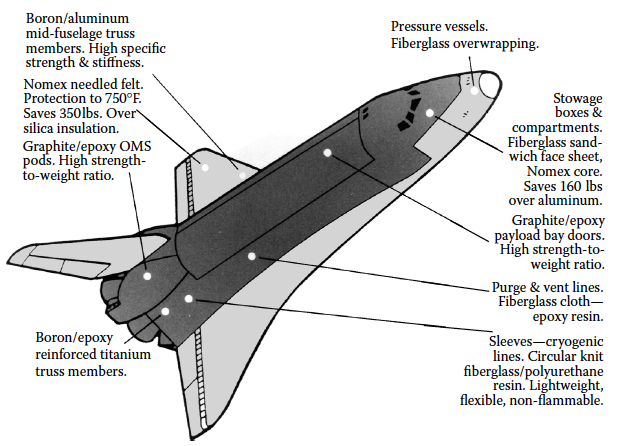
\includegraphics[width=1.0\linewidth]{fig/part0/space-shuttle.png}
				\caption{复合材料的应用一 (Graphic courtesy of M.C. Gill Corporation,
				http://www.mcgillcorp.com.)}
			\end{figure}
		\end{column}
		\begin{column}{0.4\textwidth}
			\begin{figure}
				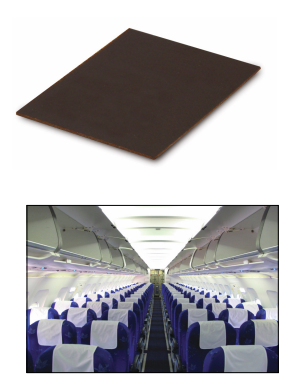
\includegraphics[width=1.0\linewidth]{fig/part0/laminate_product.png}
				\caption{ 复合材料的应用二 (Source: https://www.thegillcorp.com)}
			\end{figure}
		\end{column}
	\end{columns}
\end{frame}

\note{ 
1. Composite material gains more and more influence in commerical industry
because of its excellant mechanic performance in stiffness, stength etc., over
conventional materials.  
1. 复合材料由于其在强度和刚度等方面优良的性质广泛的应用于社会生活的方方面面。

2. Here are two examples of the use of them, the first one
is used in the space shuttle, for the main body of the space shuttle, down the
red arrow, the main reason it was chosen for weight saving and for small
mechanical and thermal deflections. 
2. 图一是复合材料应用在宇宙飞船上,在这里使用复合材料的主要原因是它能够在保持
强度的同时降低飞船自身的重量,并且在受到高温和强力冲击的时候具有较小的变形。

3. The second example is the use in the air plane,  which is because of its high
mechanical strength, heat resistant, and very low smoke evolution in a smoke.
图二是复合材料使用在飞机上,在这里使用复合材料的原因是因为复合材料的热阻效果,
和其在燃烧的时候产生 的烟雾颗粒较小。
}

\begin{frame}{什么是层合板 ? \hfill }
    \begin{columns}[c]
		\begin{column}{0.9\textwidth}
			\begin{figure}
			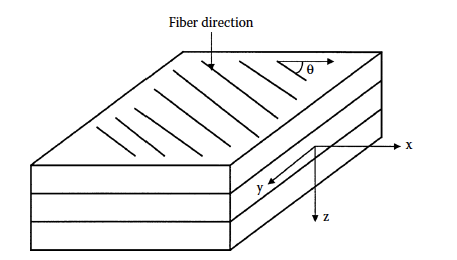
\includegraphics[width=0.85\linewidth]{fig/part0/Schematic_of_a_laminate.png}
			\caption{ Schematic of a laminate. (Source: Autar k. kaw 2006)}
			\end{figure}
		\end{column}
		%\begin{column}{0.4\textwidth}
		%\end{column}
	\end{columns}
\end{frame}
\note{ 
1. A laminate is an assembly of layers of composite materials which can be
joined to provide required engineering properties.  Figure 1 is the schematic of
a laminate. 
2. For each layer, its properies is determined by several variables: the
thickness of the layer, the fiber orientation, and engineering properites of the
material. The properitis of a laminate is determined by the combination of these
layers.  

A question arises from this is how to determine the strength of a laminate.
}

\begin{frame}{How to Predict the Strength of a Laminate ?\hfill }
    \begin{columns}[c]
	\begin{column}{0.6\textwidth}
		\begin{equation} \label{eq:force_and_moments}
			\begin{array}{l}
				\begin{aligned}
			\begin{bmatrix}
				N_x \\
				N_y \\
				N_{xy}
			\end{bmatrix}
			&=
			\begin{bmatrix}
				A_{11} & A_{12} & A_{16} \\
				A_{12} & A_{22} & A_{26} \\
				A_{16} & A_{26} & A_{66} 
			\end{bmatrix}
			\begin{bmatrix}
				\varepsilon_x^0 \\
				\varepsilon_y^0 \\
				\gamma_{xy}^0
			\end{bmatrix}   \\
			&+               
			\begin{bmatrix}
				B_{11} & B_{12} & B_{16} \\
				B_{11} & B_{12} & B_{16} \\
				B_{16} & B_{26} & B_{66} 
			\end{bmatrix}
			\begin{bmatrix}
				k_x \\
				k_y \\
				k_{xy} 
			\end{bmatrix}  \\
		\end{aligned} \\ \\
		\begin{aligned}
			\begin{bmatrix}
				M_x \\
				M_y \\
				M_{xy}
			\end{bmatrix}
			&=
			\begin{bmatrix}
				B_{11} & B_{12} & B_{16} \\
				B_{12} & B_{22} & B_{26} \\
				B_{16} & B_{26} & B_{66} 
			\end{bmatrix}
			\begin{bmatrix}
				\varepsilon_x^0 \\
				\varepsilon_y^0 \\
				\gamma_{xy}^0
			\end{bmatrix} \\ 
			&+  
			\begin{bmatrix}
				D_{11} & D_{12} & D_{16} \\
				D_{11} & D_{12} & D_{16} \\
				D_{16} & D_{26} & D_{66} 
			\end{bmatrix}
			\begin{bmatrix}
				k_x \\
				k_y \\
				k_{xy} 
			\end{bmatrix}
		\end{aligned}
			\end{array}
		\end{equation}
	\end{column}
	\begin{column}{0.4\textwidth}
		\begin{equation}
			\begin{split}
			&	\resizebox{1.0\linewidth}{!}{$A_{ij}=\sum_{k=1}^{n}(\overline{Q_{ij}})_k(h_k-h_{k-1})  i=1,2,6, j=1,2,6,$}\\
			&	\resizebox{1.0\linewidth}{!}{$B_{ij}=\frac{1}{2}\sum_{k=1}^{n}(\overline{Q_{ij}})_k(h_k^2 - h_{k-1}^2)
			i=1,2,6, j=1,2,6,$}\\
			&   \resizebox{1.0\linewidth}{!}{$D_{ij}=\frac{1}{3}\sum_{k=1}^{n}(\overline{Q_{ij}})_k(h_k^3 - h_{k-1}^3)
			i=1,2,6, j=1,2,6.$}\\
			\end{split}
		\end{equation}
	\end{column}
\end{columns}
\end{frame}

\note{
	1.  we can use this formula to compute the stress and strain for every layer
	in a laminate. In this formula, every entry in this matrix is calculate by
	the the 2, Qij are some constants relates to the composite
	material, hi and hi-1 denote local coordiate.
	2. There is another name for this equations which is called classical
	lamination theory.  which computes the stree and strain in the materail
	given the load and other conditions.  
}

\begin{frame}{How to Predict the Strength of a Laminate ?\hfill }
\begin{columns}[c]
    \begin{column}{0.4\textwidth}
		\begin{figure}
		\centering
		\resizebox{1.2\linewidth}{!}{
		\begin{tikzpicture}
			\begin{scope}
				%\draw[style=help lines] (-3,-3) grid (3,3);
				\draw (0,0) rectangle (2,3);
				\draw[->] (1.3,1.2) -- (2.6,1.2);
				\draw[->] (1.3,1.2) -- (1.3,3.4);
				\node at (2.2,1) {$X_T$};
				\node at (1.5, 3.2) {$Y_T$};
				\node at (-0.2, 0.9) {$X_C$};
				\node at (1.8, -0.2) {$Y_C$};
			\end{scope}
			\begin{scope}[xshift=6cm,yshift=1.15cm]
				%\draw[style=help lines] (-3,-3) grid (3,3);
				\draw[rotate=30] (0,0) ellipse (2cm and 1cm);
				\draw[->] (0.2,0) -- (0.2,2.2);
				\draw[->] (0.2,0) -- (1.9,0);
				\node at (1.6,-0.2) {$X_T$};
				\node at (0.3, 1.3) {$Y_T$};
				\node at (-1.6, 0) {$X_C$};
				\node at (-0.5, -1.5) {$Y_C$};
			\end{scope}
		\end{tikzpicture}
		}
		\caption{Schematic failure surfaces for maximum stress and quadratic failure
		criteria}
		\end{figure}
    \end{column}
    \begin{column}{0.6\textwidth}
		\begin{itemize}
			\item  Maximum stress failure
				\begingroup
				\small
				\begin{align*}
					SF_{MS}^k = \text{min of}
					\begin{cases}
						SF_X^k = 
						\begin{cases}
							\frac{X_t}{\sigma_{11}}, \text{ if } \sigma_{11}>0 \\
							\frac{X_c}{\sigma_{11}}, \text{ if } \sigma_{11}<0 \\
						\end{cases} \\
						SF_Y^k = 
						\begin{cases}
							\frac{Y_t}{\sigma_{22}}, \text{ if } \sigma_{22}>0 \\
							\frac{Y_c}{\sigma_{22}}, \text{ if } \sigma_{22}<0 \\
						\end{cases} \\
						SF_S^k =
						\begin{cases}
							\frac{S}{|\tau_{12}|} \\
						\end{cases} \\
					\end{cases} \textstyle{.}
				\end{align*}
				\endgroup
			\item  Tsai-wu failure theory

		 \begingroup
		 \small
		 \begin{equation*} 
		 \begin{split}
			H_1 \sigma_1  & + H_2 \sigma_2 + H_6 \tau_{12} + H_{11}\sigma_1^2 + H_{22} \sigma_2^2 \\
						  & + H_{66}  \tau_{12}^2 + 2H_{12}\sigma_1\sigma_2 < 1
		 \end{split}
		\end{equation*}
		\endgroup
		\end{itemize}
    \end{column}
\end{columns}
\end{frame}

\note{We can use these formulas to check whether a laminate  
failure or according to the stress and strain which are calculated from
above-mentioned classical lamination thoery.

These equations are called failure theory, Here we adopt two different failure theories, one is
Tsai-wu, and the other is Maximum Stress. The reason is that they have different
failure surface.

we can predict the strengh of a laminate according to classical lamination
theory and failure theory.

}

\begin{frame}{But, How to Design a Laminate?}
			\begin{itemize}
				\item Target: strength
				\item Constraints: weight cost etc.
				\item Variable: ply directiron, number of plies, material
			\end{itemize}
\end{frame}

\note{
1. But how to design it.
2. In practice, we need to tailor the structure of a laminate 
material to satisfy engineering requirements. such as the weight and cost.  
3. the layout of this  sequence is determined by several variables, the ply
thickness, the number of layers, the ply oritentation. And all these variables
are discrete in practice.  So in nature the design of laminated composite
material is a constrained optimization with discrete variables.
}


\begin{frame}{1. Methodology \hfill KIT} 
	\begin{columns}
		\begin{column}{0.65\textwidth}
			\begin{itemize}
				\item  1. formulate the objective function, assume it is $f(x)$.
				\item  2. to satisfy the constraints, adding punishment items
					$\phi_1(x),\phi_2(x),\cdots, \phi_n(x)$ 
				\item  3. reformulate the objective functions as

					$f(x)+c_1\phi_1(x)+c_2\phi_2(x)+ \cdots + c_n\phi_n(x)$
			\end{itemize}
		\end{column}
		\begin{column}{0.35\textwidth}
			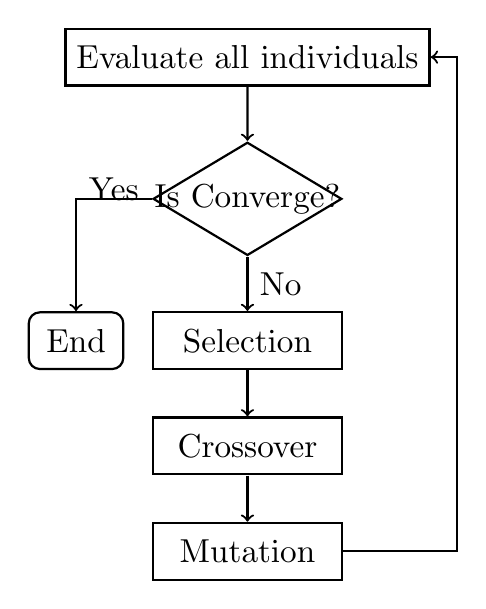
\begin{tikzpicture}[thick, scale=1.2, every node/.style={transform shape}]
	\tikzstyle{startstop} = [rectangle, rounded corners, minimum width=1.0cm,minimum height=0.6cm, text centered, draw=black]
	\tikzstyle{io} = [trapezium, trapezium left angle=70, trapezium right angle=110, minimum width=2cm, minimum height=0.6cm, text centered, draw=black]
	\tikzstyle{process} = [rectangle, minimum width=2cm, minimum height=0.6cm, text centered, draw=black]
	\tikzstyle{decision} = [diamond,minimum width=2cm, minimum height=1.2cm, draw=black]
	\node (fitness) [process] {Evaluate all individuals};
	\node[yshift=-0.5cm] (decision) [decision, below of=fitness] {} node at (decision.base) {Is Converge?};
	\node[yshift=-0.5cm] (selection) [process, below of=decision] {Selection};
	\node (crossover) [process] at ($(selection.south)+(0,-0.8cm)$) {Crossover};
	\node (mutation) [process] at ($(crossover.south)+(0,-0.8cm)$)  {Mutation};
	\node (end) [startstop] at ($(selection.west)+(-0.8cm,0cm)$) {End};

	\draw [->] (fitness) -- (decision);
	\draw [->] (decision.south) -- (selection.north) node[auto=left,pos=0.5]{No};
			   \node at ($(decision.west)+(-0.4cm, 0.1cm)$) {Yes};
	\draw [->] (selection.south) -- (crossover.north);
	\draw [->] (crossover.south) -- (mutation.north);
	\draw [->] (decision.west) -| (end.north);
	\draw [->] (mutation.east) -- ($(mutation.east)+(1.2cm,0cm)$) |-
		(fitness.east);
\end{tikzpicture}

		\end{column}
	\end{columns}
\end{frame}

\note{One of the most natural way to solve this problem is to adopt genetic
algorithm, because it doesn't require the variable to be continuous. 
This classical method works in the following step 
1. formulate the objective function. 
2. append all the constraints to the objective function as punishment items
3. reformulate the objective function.
In this formula, the coefficient c subscript 1 is coefficient whose value is from 0 to 1.

The drawback of this method is that genetic algorithm is proposed for unconstrained problem, you have to reformulate the objective function.
}



\begin{frame}{1. Methodology \hfill }
	\begin{columns}
		\begin{column}{0.6\textwidth}
			\begin{itemize}
				\item  1. formulate the objective function, assume it is $f(x)$.
				\item  2. to satisfy the constraints, maintaining different groups in the population 
				\item  3. do not change the objective function $f(x)$.
			\end{itemize}
		\end{column}
		\begin{column}{0.4\textwidth}
			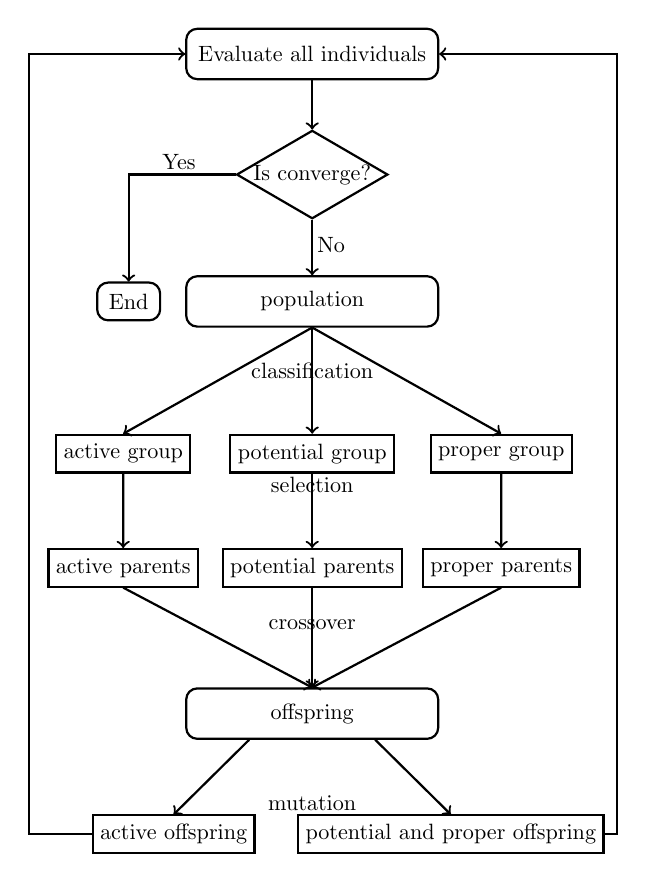
\begin{tikzpicture}[thick, scale=0.8, every node/.style={transform shape}]
	\tikzstyle{startstop} = [rectangle, rounded corners, minimum width=1.0cm,minimum height=0.6cm, text centered, draw=black]
	\tikzstyle{rec} = [rectangle,rounded corners, minimum width=4cm, minimum height=0.8cm,
	text centered, draw=black]
	\tikzstyle{subgroup} = [rectangle, minimum width=1.5cm, minimum height=0.6cm,
	text centered, draw=black]
	\tikzstyle{bigsubgroup} = [rectangle, minimum width=2.5cm, minimum height=0.6cm,
	text centered, draw=black]
	\tikzstyle{decision} = [diamond,minimum width=2.4cm, minimum height=1.4cm, draw=black]
	% population
	\node (evaluate) [rec] {Evaluate all individuals};
	\node (decision) at ($(evaluate.south)+(-0cm, -1.5cm)$)   [decision] {} node at (decision.base) {Is converge?};
	\node at  ($(decision.south)+(0.3cm, -0.4cm)$) {No};
	\node at  ($(decision.west)+(-0.9cm, 0.2cm)$) {Yes};
	\node (population) at ($(decision.south)+(-0cm, -1.3cm)$) [rec] {population};
	\node (end) at ($(population.west)+(-0.9cm, 0cm)$) [startstop] {End};
	% active group
	\node (active_group_1) at ($(population.south)+(-3cm, -2.0cm)$) [subgroup]
		{active group};
		\node (active_group_2) at ($(active_group_1.south)+(0cm, -1.5cm)$)
			[subgroup] {active parents};
		\draw[->] (decision.west) -| (end.north);
		\draw[->] (population.south) -- (active_group_1.north);
		\draw[->] (active_group_1.south) -- (active_group_2.north);
		% potential group
		\node (potential_group_1) at ($(population.south)+(0cm, -2.0cm)$) [subgroup]
				{potential group};
		\node (potential_group_2) at ($(potential_group_1.south)+(0cm, -1.5cm)$)
			[subgroup] {potential parents};
		\draw[->] (evaluate.south) -- (decision.north);
		\draw[->] (decision.south) -- (population.north);
		\draw[->] (population.south) -- (potential_group_1.north);
		\draw[->] (potential_group_1.south) -- (potential_group_2.north);
		\node at ($(potential_group_1.north)+(0cm, 1.0cm)$) {classification };
		\node at ($(potential_group_2.north)+(0cm, 1.0cm)$) {selection};
		% proper group
		\node (proper_group_1) at ($(population.south)+(3cm, -2.0cm)$) [subgroup]
			{proper group};
		\node (proper_group_2) at ($(proper_group_1.south)+(0cm, -1.5cm)$)[subgroup]
			{proper parents};
		\draw[->] (population.south) -- (proper_group_1.north);
		\draw[->] (proper_group_1.south) -- (proper_group_2.north);
		% crossover
		\node (after_cross_over) at ($(potential_group_2.south)+(0cm, -2.0cm)$) [rec] {offspring};
		\node  at ($(after_cross_over.north)+(0cm, 1.0cm)$)  {crossover};
		\draw[->] (active_group_2.south) -- (after_cross_over.north);
		\draw[->] (potential_group_2.south) -- (after_cross_over.north);
		\draw[->] (proper_group_2.south) -- (after_cross_over.north);
		% mutation
		\node (active_group_3) at ($(after_cross_over.south)+(-2.2cm, -1.5cm)$)
			[subgroup] {active offspring};
		\node at ($(after_cross_over.south)+(0cm, -1.0cm)$) {mutation};
		\draw[->] ($(after_cross_over.south)+(-1cm,0cm)$)--(active_group_3.north);
		\node (poteni_and_prop) at ($(after_cross_over.south)+(2.2cm, -1.5cm)$)
			[bigsubgroup] {potential and proper offspring};
		\draw[->] ($(after_cross_over.south)+(1cm,0cm)$)--(poteni_and_prop.north);

		% final draw
		\draw[->] (poteni_and_prop.east) --($(poteni_and_prop.east) + (0.2cm,0cm)$) |- (evaluate.east);
		\draw[->] (active_group_3.west) -- ($(active_group_3.west) + (-1cm,0cm)$)
			|- (evaluate.west);
		\end{tikzpicture}

		\end{column}
	\end{columns}
\end{frame}

\note{The general flowchart of the proposed genetic algorithm is as shown in
	Fig4. 
	Compared with the classical GA, there are two differences:
	
	1. first, classify the population into three different groups according to the
	constraints, active group, potential group and proper group. we will explain
	these terminology later.
	2. second, the mutation operator for active group and potential, proper
	group is different. For the active group, the mutation follows the
	traditional pattern; we will adopt new mutation technique for the potential
	and proper group.
 }

\begin{frame}{Definition \hfill}
		\begin{itemize}
			\item An individual is active if its constraint value is far smaller than the
				threshold. A group is consist of
				active individuals are called as active group.
			\item An individual is potential if its constraint value is  close but smaller than the
				thresold. The corresponding group is
				refered as potential group.
			\item An individual is proper if it satisfy all the constraints. Its
				counterpart group is written as proper group.
		\end{itemize}
\end{frame}

\note{Here are some definition and terminology:
The role of different group is different. The role of active group is to
maintain the diversity of the mating pool. The role of potential group is to
find possible solutions. In the proper group, they are  the individual that we want.}



\begin{frame}{Techniques for Mutation \hfill KIT}
    \begin{columns}[c]
    \begin{column}{1\textwidth}
		$\text{md} = [CT_1, \cdots, CT_{n-1}, CT_n] -  [ICV_1, \cdots, ICV_{n-1},
		ICV_n]$ \\
		\begin{itemize}
			\item  md means mutation direction.
			\item  $CT_i$ denotes the i-th constraint, such as weight, strength ratio.
			\item  $ICV_i$ denotes individual's i-th constraint value, such as,  weight, strength ratio 
				of current individual.
		\end{itemize}

    \end{column}
\end{columns}
\end{frame}

\note{The second technique in the proposed genetic algorithm is self-adaptive mutation
	operator, which means it can adjust the mutation according to the
	constraint value.  In this formula, the CTn represents threshold, ICVn
	denotes the corresponding individual's constraint value.  We get a mutation
	vector from this formula, which can be used to direct the mutation of the
chromosome.}


\begin{frame}{1. Methodology \hfill KIT}
    \begin{columns}[c]
	\begin{column}{1\textwidth}
		\begin{itemize}
			\item length mutation =  
				\[
				  \begin{cases}
					  LMC*[0, \sum_{i=1}^{N}{md_i}] & \text{if $\sum_{i=1}^{N}{md_i} > 0$} \\
					  LMC*[\sum_{i=1}^{N}{md_i}, 0] & \text{if $\sum_{i=1}^{N}{md_i} < 0$} \\
				  \end{cases}
				\] \\
				LMC stands for length mutation coefficient, it's a positive integer.
			\item $P(AM)$ = 
				\[
				  \begin{cases}
					0.5, \text{ AM = }[0,AMC \sum_{i=1}^{N}{(|CT_i-CV_i|)}] \\ 
					0.5, \text{ AM = }[ AMC \sum_{i=1}^{N}{(-|CT_i-CV_i|)},0]
				  \end{cases}
				\] \\
				AMC stands for angle mutation coefficient.
		\end{itemize}
	\end{column}
\end{columns}
\end{frame}


\note{The self-adaptive mutation is consist of two parts: length mutation and angle mutation.
	for the length mutation, we increase the length of the chromosome when the
	sum of entries in the mutation is great than zero,  this is because the
	bigger the length is, the more possible it satisfy the constraint. 
	For the angle mutation, we just
	random change the angels with probability 0.5, because there is no clear
	relation between the ply oritentation and the strength.
}



\note{
		 To overcome the drawback of traditional genetic algorithm in the
			design of laminated sequence, and propose a new genetic algorithm
			framework with two techniques for solving constrained problem
			optimization.
		 To improve the performance and efficient of the design laminate sequence, compared with the other optimization method.
		 To obtain feasible solutions for single-constrained or multiple constrained design of laminate sequence. 

The first is overcome the drawback of traditional genetic algorithm in the
design of a laminate.
The second is to improve the performance and efficient of the design of a
laminate.
The third is to find feasible solutions for single-constrained and multiple
constrained problem.

Therefore, we proposed a new genetic algorithm with two Techniques, the
first is mating pool classification, and the second is self-adaptive mutation
operator. The advantage of this method is that We don't need to reformulate the
objective function.}

\begin{frame}{1. Result \hfill} 
	%\begin{table}[!htb]
\caption{The optimum lay-ups for the loading $N_x=1e6$ N}
\centering
\begin{adjustbox}{width=1\textwidth}
\begin{tabular}{c|cc|cc}
	\toprule
	Cross Ply $[0_M/90_N]$         & \multicolumn{2}{c}{Choudhury and Mondal's} & \multicolumn{2}{c}{Current Research} \\
	\midrule																								  
	 Material       &  Glass-Epoxy & Graphite-Epoxy  & Glass-Epoxy & Graphite-Epoxy      \\ 
	      M         &  68          &    17           &  78		    &  18             \\
	      N         &  72          &    18           &  28		    &  8              \\
no. of lamina(n)    &  140         &    35           &  106	    &  26                     \\
         SR         &  2.01        &    2.10         &  2.03	    &  2.16            \\
     weight         &  9.10        &    1.84         &  6.89	    &  102.5           \\
	\bottomrule
\end{tabular}
\end{adjustbox}
\label{tab:comparsion}
\end{table}

	\begin{table}
\caption{Comparison of experiment results of Choudhury and
Mondal's and current study under in-plane loading
$N_x=1e6$ N. The results of present study is from previous experiment.}
\centering
\begin{adjustbox}{width=1\textwidth}
	\begin{tabular}{c|cc|cc}
		\toprule
		Cross Ply $[0_M/90_N]$         & \multicolumn{2}{c}{Choudhury and Mondal's study} & \multicolumn{2}{c}{Present study} \\
		\midrule																								  
		 Material       &  Glass-Epoxy & Graphite-Epoxy  & Glass-Epoxy & Graphite-Epoxy      \\ 
			  M         &  68          &    17           &  76		    &  19             \\
			  N         &  72          &    18           &  49		    &  2              \\
	no. of lamina(n)    &  140         &    35           &  125	        &  21                     \\
			 SR         &  2.01        &    2.10         &  2.08	    &  2.15            \\
		 weight         &  9.10        &    1.84         &  8.12	    &  1.10           \\
		 cost           &  140         &    87.50        &  125	        &  53           \\
		\bottomrule
	\end{tabular}
\end{adjustbox}
\label{tab:comparsion}
\end{table}


\end{frame}
\note{We also compare our work with other results in other literature.
	As you can see from the table, we obtained better results for both cases.
}


\note{We have three conclusions from this chapter:
	The first is that the proposed genetic algorithm can be used to guide the
	design of laminated structure with one or multiple constraints without
	modifying the objective function.
	The second is mating pool classification and self-adaptive mutation play an
	important role during the optimization process, the length muation
	coefficient can be used to control the converge speed of this algorithm.
	This method will have a fine-grained search with a small length mutation
	coefficient.

	The proposed algorithm outperformed or provided an alternative feasible
	solution compared with other literature.  The proposed genetic algorithm can
	be used to guide the design of laminated structure with one or multiple
	constraints without modifying the objective function.  The simulation
	results have shown that the two technique: mating pool classification and
	self-adaptive mutation play an important role during the optimization
	process, the length muation coefficient can be used to control the converge
	speed of this algorithm.  The proposed algorithm is able to outperform or
	provide an alternative solution compared with other literature.
}


\begin{frame}{发表论文}
	\begin{center}
		\begin{itemize}
			\item Huiyao Zhang, Atsushi Yokoyama. 2021. A Technique for Constrained Optimization of Cross‑ply Laminates Using a New
				Variant of Genetic Algorithm. International Journal of Advanced Computer Science and Applications, 12(6): 760‑767.
			\item Huiyao Zhang, Atsushi Yokoyama. 2022. Optimum Design of Laminated Composites for Minimum Thickness by a Variant
				of Genetic Algorithm. Journal of Textile Engineering(accepted)
		\end{itemize}
	\end{center}
\end{frame}

\note{Chapter Four focuses on using an alternative method to predict the strength of a laminated composite material.

		 To reduce the computation cost in the strength prediction of
			laminated structure with classical lamination theory and failure
			theory.
		 To simplify the procedure of strength prediction calculation.
		 To provide a data-driven method to compute the strength ratio instead of the traditional analytical method.
}




\begin{frame}{问题二: 如何预测层合材料的强度? }
	\begin{center}
		\begin{figure}
			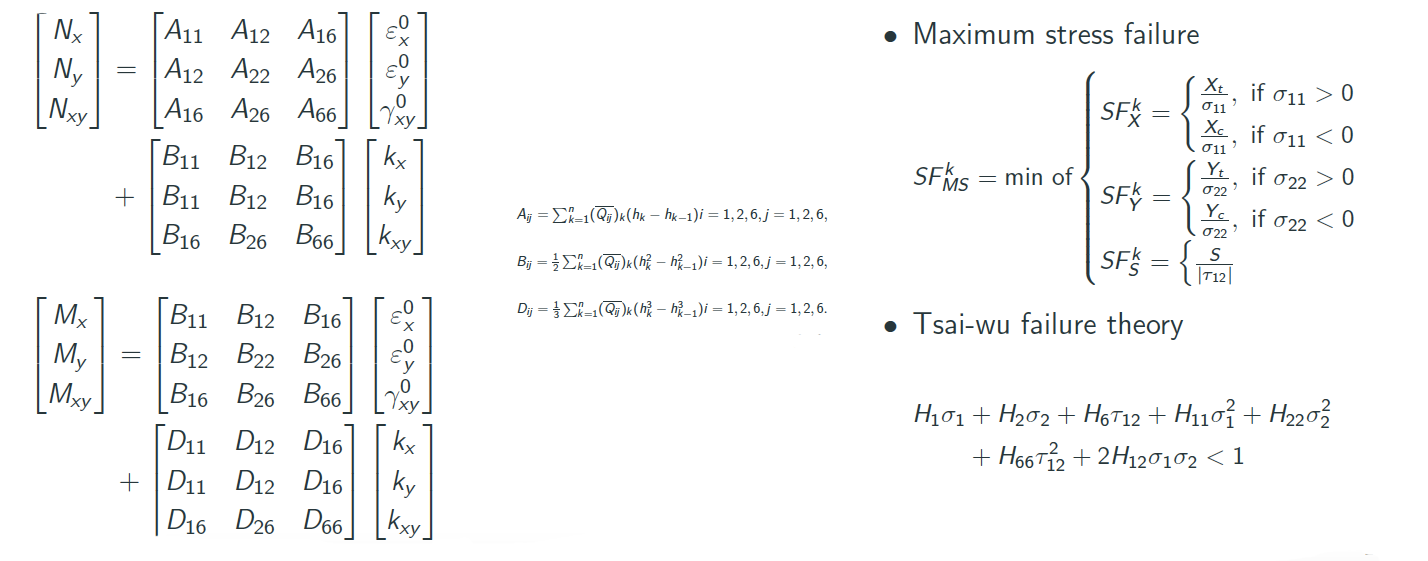
\includegraphics[width=1\textwidth]{fig/part3/formula_for_stenght_calculation.png}
		\end{figure}
	\end{center}
\end{frame}

\note{
    我们可以使用这个幻灯片中的公式来计算层合材料的强度,这些公式有一个名字叫做,
	经典的层合理论和纤维失效理论,它是使用解析的方法,根据经典的力学模型计算应力和应变来预测材料的强度。
	这种方法存在的一个问题是,她的步骤比较繁琐,而且这个算法的时间复杂度比较高,因为包含了
	大量的矩阵乘法和积分的运算。因此,我推荐使用数据驱动的方法,也就是神经网络来预测
	复合材料的强度

Another problems arises from a laminate is the the strength prediction.
	The traditional way of doing this follows a two-step precedure: first,
	calculate the stress and strain within the laminated composite material by
	using of classical lamination theory. Second use failure theory to check the
	corresponding material failure or not. The first drawback of this method is
	that the computation cost is high because of the involvment of matrix
	multplication and interal operation and interal operation.  There we propose
	to use evolutionary artificial neural network to predict the strenght of
	angle ply laminate.}

\begin{frame}{如何设计网络的拓扑结构?}
	
\begin{figure}
	\begin{center}
\begin{tikzpicture}
[ plain/.style={ draw=none, fill=none, }, remember picture, net/.style={ matrix of nodes, nodes={ draw, circle,
    inner sep=7.5pt
    },
  nodes in empty cells,
  column sep=-10.5pt,
  row sep=0.8cm
  }
]
%\draw[help lines] (-3cm,-6cm) grid (6cm,3cm);
\matrix[net] (mat)
{
              & |[plain]| &           & |[plain]|  &           & |[plain]| &           &  |[plain]|      &               \\
    |[plain]| &           & |[plain]| &            & |[plain]| &           & |[plain]| &                 & |[plain]|     \\ 
    |[plain]| & |[plain]| &           & |[plain]|  &           & |[plain]| & 	  	   &  |[plain]|      & |[plain]|     \\ 
  };

  \node at ($(mat-1-1.west)+(-16pt,0)$) {输入层: };
  \node at ($(mat-2-2.west)+(-24pt,0)$) {隐藏层:};
  \node at ($(mat-3-2.west)+(-24pt,0)$) {输出层:};
  \node at (mat-1-1.base) {$i_1$};
  \node at (mat-1-3.base) {$i_2$};
  \node at (mat-1-5.base) {...};
  \node at (mat-1-7.base) {$i_{n-1}$};
  \node at (mat-1-9.base) {$i_{n}$};
  \node at (mat-2-2.base) {$h_1$};
  \node at (mat-2-4.base) {$h_2$};
  \node at (mat-2-6.base) {$...$};
  \node at (mat-2-8.base) {$h_{m}$};
  \node at (mat-3-5.base) {$...$};

 \foreach \a in {1,3}{
    \foreach \b in {2,6}{
        \draw[->] (mat-1-\a.south) -- (mat-2-\b.north);
     }
  }
 \foreach \a in {3,7,9}{
    \foreach \b in {4,8}{
        \draw[->] (mat-1-\a.south) -- (mat-2-\b.north);
     }
  }

 \foreach \c in {2,4,6,8}{
    \foreach \d in {3,5,7}{
 		\draw[->] (mat-2-\c.south) -- (mat-3-\d.north);
	}
 }
\end{tikzpicture}
\caption{神经网络模型}
\end{center}
\end{figure}

\end{frame}

\note{we proposed the following general neural network to solve the strength
	prediction. 
	1. Neurons in the hidden layer are treated as feature extractor, which means
	it learn something from the inputs, neurons in the hidden layer are partly
	connect with the inputs, because uncecessary connection will casue
	overfitting. 
	and we treat neurons in the hidden layer
	as the feature learned from the inputs. Therefore the neurons in the outputs
	layer should be fully connected with the previous layer.}

\begin{frame}{2. Methodology \hfill }
	\begin{figure}
		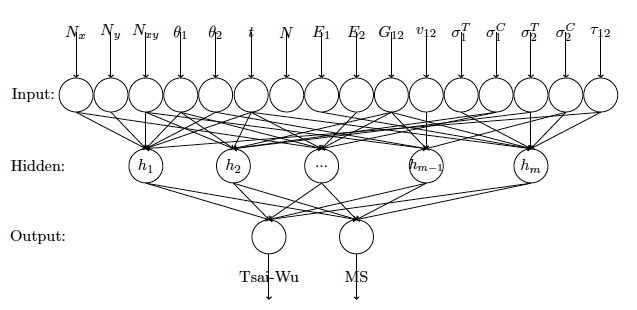
\includegraphics[width=0.9\textwidth]{fig/a0_figure_ann_for_clt_architecture.png}
		\caption{General neural network for prediction the strength of an angle ply laminate.}
	\end{figure}
\end{frame}

\note{To calculate the Based on the general neural network architecture, we proposed the
	following structure to predict the strength of angle ply structure. There
	are two outputs, which are tsai wu strength ratio, and maximum strength
	ratio.
	There are 16 inputs, which are consist of four parts:
	the first part is the loading that imposed on the laminate, Nx, Ny, Nxy
	the second part is the sequence of the angle ply laminate, which are two
	ply oritenation, ply thickness, and the number of plies.
	the third part is the four engineering  constants, E1,E2,G12, v12
	Traverse elastic modulus 
	Major Poisson's ratio 
	Shear modulus 
	the fourth part is five constants about the failure properties of the material: 
Ultimate longitudinal tensile strength 
Ultimate longitudinal compressive strength 
Ultimate transverse tensile strength 
Ultimate transverse compressive strength 
Ultimate in-plane shear strength 
Longitudinal elastic modulus 
}

\begin{frame}{2. Methodology \hfill }
	\begin{figure}
		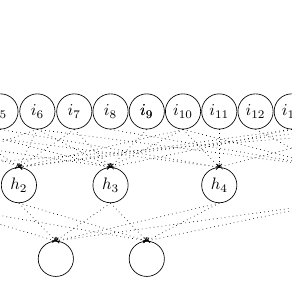
\begin{tikzpicture}
	[ p/.style={ draw=none, fill=none}, 
	  remember picture, 
	  net/.style={ matrix of nodes, nodes={ draw, circle, inner sep=7.5pt },
	  nodes in empty cells,
	  column sep=-10.5pt,
	  row sep=0.8cm, 
	  }
	]
	\useasboundingbox (-1.5,-1.1) rectangle (1.5,2);
	\scope[transform canvas={scale=0.6}]
\matrix[net] (mat)
{
		  & |[p]| &  & |[p]| &  & |[p]| &  & |[p]| &  & |[p]| &  & |[p]| &  & |[p]| &  & |[p]| &  &
			|[p]| &  & |[p]| &  & |[p]| &  & |[p]| &  & |[p]| &  & |[p]| &  & |[p]| &  & |[p]|    \\
	 |[p]| & |[p]| & |[p]| &  |[p]| &        & |[p]| & |[p]| & |[p]| &|[p]| &       & |[p]| &  |[p]| & |[p]| &
	 |[p]| &       & |[p]| &  |[p]| &  |[p]| & |[p]| & |[p]| &       &|[p]| & |[p]| & |[p]| & |[p]|
		   & |[p]| &       &  |[p]| &  |[p]| & |[p]| & |[p]| & |[p]| &|[p]| \\ 
	 |[p]| &  |[p]| & |[p]|  &  |[p]| & |[p]|  &  |[p]| &  |[p]| &  |[p]| & |[p]| & |[p]| & |[p]| &       & |[p]|
		   &  |[p]| & |[p]|  &  |[p]| &        &  |[p]| &  |[p]| &  |[p]| & |[p]| & |[p]| & |[p]| & |[p]| &     |[p]|
		   &  |[p]| & |[p]|  &  |[p]| & |[p]|  &  |[p]| &  |[p]| &  |[p]| \\ 
	  };
	  \node at (mat-1-1.base)  {$i_1$};
	  \node at (mat-1-3.base)  {$i_2$};
	  \node at (mat-1-5.base)  {$i_3$};
	  \node at (mat-1-7.base)  {$i_4$};
	  \node at (mat-1-9.base)  {$i_5$};
	  \node at (mat-1-11.base)  {$i_6$};
	  \node at (mat-1-13.base)  {$i_7$};
	  \node at (mat-1-15.base)  {$i_8$};
	  \node at (mat-1-17.base)  {$i_9$};
	  \node at (mat-1-17.base)  {$i_9$};
	  \node at (mat-1-19.base)  {$i_{10}$};
	  \node at (mat-1-21.base)  {$i_{11}$};
	  \node at (mat-1-23.base)  {$i_{12}$};
	  \node at (mat-1-25.base)  {$i_{13}$};
	  \node at (mat-1-27.base)  {$i_{14}$};
	  \node at (mat-1-29.base)  {$i_{15}$};
	  \node at (mat-1-31.base)  {$i_{16}$};

	  \node at (mat-2-5.base)  {$h_1$};
	  \node at (mat-2-10.base) {$h_2$};
	  \node at (mat-2-15.base) {$h_3$};
	  \node at (mat-2-21.base) {$h_4$};
	  \node at (mat-2-27.base) {$h_5$};
		 \foreach \a in {1,3,5,7,9,11,31}{
				\draw[->,dotted] (mat-1-\a.south) -- (mat-2-5.north);
			 }
		 \foreach \a in {5,7,11,13,19,25,27}{
				\draw[->,dotted] (mat-1-\a.south) -- (mat-2-10.north);
			 }
		 \foreach \a in {1,7,11,13,17,19,25}{
				\draw[->,dotted] (mat-1-\a.south) -- (mat-2-15.north);
			 }
		 \foreach \a in {5,9,19,21,29}{
				\draw[->,dotted] (mat-1-\a.south) -- (mat-2-21.north);
			 }
		 \foreach \a in {11,15,19,23,27,29,31}{
				\draw[->,dotted] (mat-1-\a.south) -- (mat-2-27.north);
			 }
		 \foreach \c in {5,10,15,21,27}{
			\foreach \d in {12,17}{
				\draw[->,dotted] (mat-2-\c.south) -- (mat-3-\d.north);
			}
 }
 \endscope
\end{tikzpicture}

		\caption{Example of proposed architecture.}
		\label{fig:example}
	\end{figure}
	\begin{table}
		\centering
		\caption{The binary representation of Figure \ref{fig:example}.
		}
		\begin{adjustbox}{width=0.8\textwidth}
		\begin{tabular}{l|cccc cccc cccc cccc | cc}
			\toprule
				 Nodes  & $i_1$ & $i_2$ & $i_3$ & $i_4$ & $i_5$ & $i_6$ & $i_7$ & $i_8$ & $i_9$ & $i_{10}$ & $i_{11}$ & $i_{12}$ & $i_{13}$ & $i_{14}$ & $i								_{15}$ & $i_{16}$ & f & f\\
			\midrule
				   	$h_1$ & 1  & 1 & 1  & 1  & 1 & 1 & 0 & 0  & 0 & 0 & 0 & 0  & 0 & 0  & 1 & 1 & 0 & 0\\
					$h_2$ & 0  & 1 & 1  & 1  & 0 & 0 & 0 & 1  & 0 & 0 & 1 & 1  & 0 & 0  & 0 & 0 & 1 & 1\\
					$h_3$ & 1  & 0 & 0  & 1  & 0 & 1 & 1 & 0  & 1 & 1 & 0 & 0  & 1 & 0  & 0 & 0 & 0 & 0\\
					$h_4$ & 0  & 0 & 1  & 0  & 1 & 0 & 0 & 0  & 0 & 1 & 0 & 1  & 0 & 0  & 1 & 0 & 0 & 1\\
					$h_5$ & 0  & 0 & 0  & 0  & 0 & 1 & 0 & 1  & 0 & 1 & 0 & 1  & 0 & 1  & 1 & 1 & 0 & 1\\
			\bottomrule
			\end{tabular}
		\end{adjustbox}
\end{table}



\end{frame}

\note{In order to adopte genetic algorithm for neural network revolution, we
	need to represent this neural network with a chromosome. Table 8 is the
	binary representation of the above neural network, with one row
	representing a neuron.  for every neuron, if there exist a connection
	between the neuron and the inputs, we denote with 1, otherwise, it is
zero.The last two column is the code for active function.}


\begin{frame}{2. Methodology \hfill }
	\begin{columns}
		\begin{column}{0.8\textwidth}
			\begin{figure}
				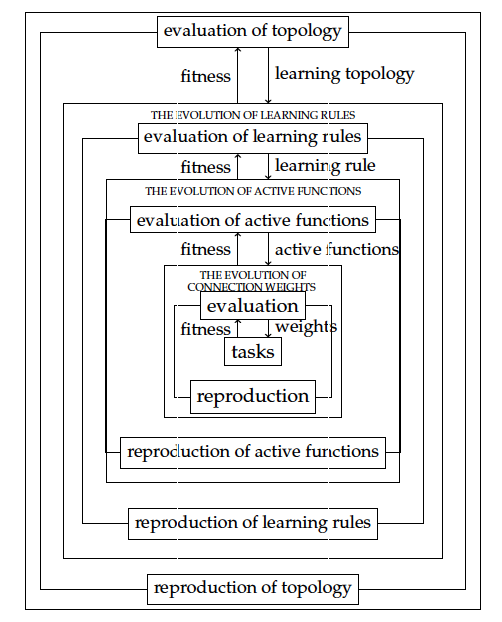
\includegraphics[width=0.7\linewidth]{fig/part3/architecture_of_evolution.png}
				\caption{The evolution of this neural network}
			\end{figure}
		\end{column}
	\end{columns}
\end{frame}

\note{This neual network is neural network has four parts of evolution:}

\begin{frame}{2. Methodology \hfill }
	\begin{figure}
	\centering
	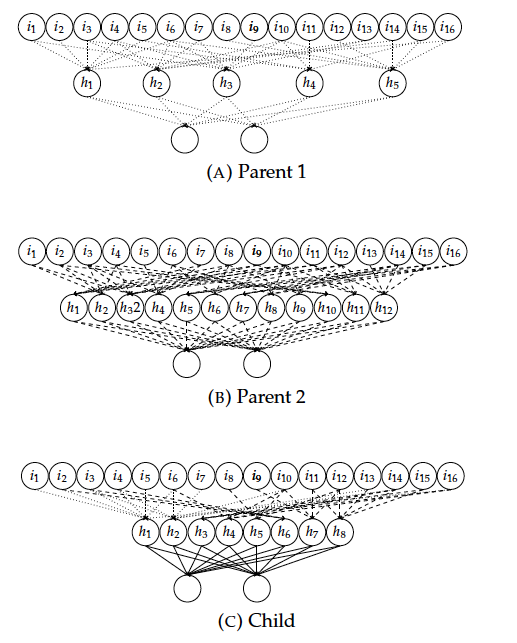
\includegraphics[scale=0.3]{fig/part3/interitance.png}
	\caption{Examples of three ANNs, with (a) and (b) as parent ANNs, and (c) as
	the child of (a) and (b). }
		\label{fig:anns}
	\end{figure}
\end{frame}

\note{We also present the crossover operator about the neural network. child c
inherits the connection relationship part from parent 1 denoted by the darker
dashed lines,and the rest from parent 2 denoted by the gray dashed line}


\begin{frame}{2. Preparation of Training Data \hfill KIT}
	\begin{table}	
	\caption{Part of train dataset}
	\resizebox{10cm}{!}{
	\begin{tabular}{cccc|cc}
		\toprule
		\multicolumn{4}{c}{\textbf{Input}} &  \multicolumn{2}{c}{\textbf{Output}} \\
		\midrule
		Load  &  \makecell{Laminate \\ Structure }  & \makecell{Material \\ Property} & \makecell{Failure \\  Property}  & MS & Tsai-Wu \\
		\midrule

		-70,-10,-40,  & 90,-90,4,1.27, & 38.6,8.27,0.26,4.14,  & 1062.0,610.0,31,118,72,  & 0.0102, & 0.0086 \\
		-10,10,0,     & -86,86,80,1.27,& 181.0,10.3,0.28,7.17, & 1500.0,1500.0,40,246,68, & 0.4026, & 2.5120 \\
		-70,-50,80,   & -38,38,4,1.27, & 116.6,7.67,0.27,4.173,& 2062.0,1701.0,70,240,105,& 0.0080, & 0.0325 \\
		-70,80,-40,   & 90,-90,48,1.27,& 38.6,8.27,0.26,4.14,  & 1062.0,610.0,31,118,72,  & 0.0218, & 0.1028 \\
		-20,-30,0,    & -86,86,60,1.27,& 181.0,10.3,0.28,7.17, & 1500.0,1500.0,40,246,68, & 0.6481, & 0.9512 \\
		0,-40,0,      & 74,-74,168,1.27,& 181.0,10.3,0.28,7.17,& 1500.0,1500.0,40,246,68, & 1.3110, & 3.9619 \\
		\bottomrule
		\end{tabular}
	}
\end{table}

\end{frame}

\note{Since it is impossible to obtain enough training data from experiment,
therefore, we generate the training data by use of classical lamination theory and
failure theory. Table 11 shows part of our training data, in which the load
varys from -200 to 200 MP a for every component. the ply orientation varies
from -90 to 90. We use three different composite materail. The training data is
randomly sampled from this space. After obtain the two ouputs, we need
normalize the training data for the learning of the neural network.}

\begin{frame}{2. Result \hfill }
	\begin{columns}
		\begin{column}{0.6\textwidth}
			\begin{table}
	\centering
	\caption{Comparsion of Fully-connected Neural Network and GA-based Neural
	Network}
	\label{tab:simu}
		\resizebox{\textwidth}{!}{
	\begin{tabular}{ccc}
		\toprule
		Model     & Training Error & Validation Error   \\
		\midrule
		Fully-connected ANN &   0.051 & 0.050\\
		GA-based ANN       &   0.054 & 0.055\\
		\bottomrule
	\end{tabular}
}
\end{table}

		\end{column}
	\end{columns}
	\begin{center}
		\begin{itemize}
			\item Huiyao Zhang, Atsushi Yokoyama. 2021. Predicting Strength Ratio of Laminated Composite Material with Evolutionary
				Artificial Neural Network. International Journal of Advanced Computer Science and Applications, 12(6): 11‑18.
		\end{itemize}
	\end{center}
\end{frame}

\note{
We also trained a neural network which has the same architecture as the neural
network that we obtained from genetic algorithm. The only difference is that
neurons in the hidden layer are fully connected with the inputs.
}


\note{
		 Neural network can be adopted to predict the strength of laminated composite material instead of the classical analytical approach.
		 GA-based neural network outperformed fully-connected neural network in the strength prediction.

	The summary of this chapter is as following:
		Neural network can be adopted to predict the strength of laminated composite material instead of the classical analytical approach.
		GA-based neural network outperformed fully-connected neural network in the strength prediction.
}

\begin{frame}
	\begin{center}
		\Huge{Thank You}
	\end{center}
\end{frame}


\end{document}



